\documentclass[aspectratio=169,9pt]{beamer}
\mode<presentation> 
\usepackage[utf8]{inputenc}
\usepackage{sansmathaccent} %Für equations
\usepackage{amsmath}
\usepackage{tikz}
\usepackage{multicol}
\usepackage{cancel}
\usepackage{relsize}
\usepackage{graphicx}
\usepackage[table]{xcolor}
\usepackage{fontawesome5}
\usepackage{enumitem}
\usepackage{setspace}
\usepackage[labelfont={bf},font={color=black!40,footnotesize},tablename={Tabelle},figurename={Abbildung}]{caption}
\usetikzlibrary{positioning, arrows.meta, calc, matrix}
\usefonttheme[onlymath]{serif}
%\makeatletter
%\makeatother

\usetikzlibrary{patterns, arrows.meta, calc}
\usepackage{pgfplots}
\pgfplotsset{compat=1.18}
\usetikzlibrary{intersections, pgfplots.fillbetween}\usetikzlibrary{intersections, pgfplots.fillbetween}
\rowcolors{2}{miugray!30}{miugray!10}

\usetheme{Madrid}  %% Themenwahl
\useoutertheme{split} % Alternatively: miniframes, infolines, split
%\useinnertheme{circles}


\setbeamertemplate{itemize item}{\color{miugray}$\blacksquare$}
\setbeamertemplate{itemize subitem}{\color{uniblau}$\bullet$}



%\newcommand{\metermilli}{\mskip3mu \text{mm}}
\newcommand{\cm}{\mskip3mu \text{cm}}
\newcommand{\m}{ \text{m}}
\newcommand{\lite}{ \text{l}}
\newcommand{\kg}{ \text{kg}}
\newcommand{\g}{ \text{g}}
\newcommand{\km}{ \text{km}}
\newcommand{\h}{ \text{h}}
\newcommand{\s}{ \text{s}}
\newcommand{\tonne}{ \text{t}}


\newcommand{\RA}{$\rightarrow$~}
\newcommand{\pp}{\par \vspace*{2mm}}
\newcommand{\ppbig}{\par \vspace*{4mm}}

\definecolor{miudiutex}{HTML}{1d2926}
\definecolor{miugray}{HTML}{b4cccf}
\definecolor{miugray2}{HTML}{4d7365}
\definecolor{white2}{HTML}{f5f7f8}
\definecolor{red}{HTML}{cf1f5c}
\definecolor{green}{HTML}{00A36C}
\definecolor{delphinidin}{HTML}{315794}
\definecolor{uniblau}{HTML}{004e9f}
\definecolor{unigelb}{HTML}{fcba00}
\definecolor{unigrau}{HTML}{909085}
\definecolor{pelargonidin}{HTML}{b33807}
\definecolor{cyanidin}{HTML}{ba0746}
\definecolor{paeonidin}{HTML}{d15ca6}
\definecolor{petunidin}{HTML}{b56fed}
\definecolor{malvidin}{HTML}{8a2d8c}

%\setbeamercolor{palette primary}{bg=pelargonidin!35,fg=white}
%\setbeamercolor{palette secondary}{bg=delphinidin!45,fg=white}
\setbeamercolor{palette primary}{bg=uniblau!70,fg=white}
\setbeamercolor{palette secondary}{bg=uniblau!45,fg=white}
\setbeamercolor{palette tertiary}{bg=unigelb!70,fg=unigrau}
\setbeamercolor{palette quaternary}{bg=miugray,fg=white}
\setbeamercolor{structure}{fg=black} % itemize, enumerate, etc
\setbeamercolor{section in toc}{fg=red} % TOC sections

\setbeamersize{text margin left=1cm,text margin right=1cm}


\useinnertheme{tcolorbox} 
\newcommand{\goodtk}[2]{
\begin{tcolorbox}[
	enhanced,
	colframe=uniblau!75,
	sharp corners,
	boxsep=5pt,
	title=\bfseries \sffamily #1,
	colback=white,
	coltitle=black,
	attach boxed title to top text left={yshift=-\tcboxedtitleheight/2},
	boxed title style={colback=white,colframe=white}
]
	#2
	\end{tcolorbox}
}
	
\newcommand{\antwort}[1]{
\begin{tcolorbox}[
	enhanced,
	colframe=unigrau!65,
	sharp corners,
	boxsep=1pt,
	colback=white,
	coltitle=black,
]
	#1
	\end{tcolorbox}
}


\title{7. Übung}
\author{PD Dr. Helene Loos}
\date{\today}

\begin{document}
%\maketitle
\small



\begin{frame}
\begin{center}

\LARGE Übung 8  \par \normalsize
Prozessbezogene Lebensmitteltechnologie
\end{center}
\small
\end{frame}



\begin{frame}

\begin{minipage}{.5\textwidth}


{\color{miugray}$\blacksquare ~$} \textbf{Aufgabe 1} \par \vspace*{2mm}
Eine Probe Cornflakes hat einen gravimetrischen Wassergehalt von 7,5\% bezogen auf die
Feuchtmasse. Berechnen Sie den gravimetrischen Wassergehalt bezogen auf die
Trockenmasse.



\end{minipage}%
\hspace*{4mm}
\begin{minipage}{.5\textwidth}
\antwort{
\uncover<2->{
\begin{align*}
\frac{7,5}{92,5}  \qquad = \qquad 0,081 \qquad \hat{=} \qquad 8,11 \%
\end{align*}
}
}
\end{minipage}%

\end{frame}




\begin{frame}

\begin{minipage}{.5\textwidth}


{\color{miugray}$\blacksquare ~$} \textbf{Aufgabe 2} \par \vspace*{2mm}
Eine Charge Cornflakes hat einen gravimetrischen Wassergehalt von 21,2\% bezogen auf die
Trockenmasse. Berechnen Sie den gravimetrischen Wassergehalt bezogen auf die
Feuchtmasse.



\end{minipage}%
\hspace*{4mm}
\begin{minipage}{.5\textwidth}
\antwort{
\uncover<2->{
\begin{align*}
\frac{21,2}{121,2} \qquad = \qquad 17,5 \%
\end{align*}
}
}
\end{minipage}%


\end{frame}



\begin{frame}
\begin{minipage}{.5\textwidth}


{\color{miugray}$\blacksquare ~$} \textbf{Aufgabe 3} \par \vspace*{2mm}
1.200 g einer 24\%igen Lösung sollen durch Eindampfen auf 60\% konzentriert werden. Wie viel
Gramm Wasser sind zu entziehen?

\end{minipage}%
\hspace*{4mm}
\begin{minipage}{.5\textwidth}
\antwort{
Mischungsgleichung

Mit: $x_1 = 0\%$ ; $x_2 = 60\%$ ; $x_3 = 24\%$ ; \par \hspace*{5mm} $m_1 = ?$ ; $m_2 = m_3 - m_1$ ; $m_3 = 1200$

\begin{align*}
\uncover<2->{m_1x_1 + m_2x_2 &= m_3x_3 \\}
\uncover<3->{m_1x_1 + m_3x_2 - m_1x_2 &= m_3x_3 \\}
\uncover<4->{m_1x_1 - m_1x_2 &= m_3x_3 - m_3x_2 \\}
\uncover<5->{m_1(x_1-x_2) &= m_3(x_3-x_2) \\}
\uncover<6->{m_1 &= \frac{m_3(x_3-x_2)}{(x_1-x_2)} \\}
\uncover<7->{m_1 &= \frac{1200(0,24-0,6)}{0-0,6}\\
 &= 720}
\end{align*}
\uncover<8->{
Daher müssen 720 g Wasser entzogen werden. 
}
}
\end{minipage}%

\end{frame}



\begin{frame}

\begin{center}
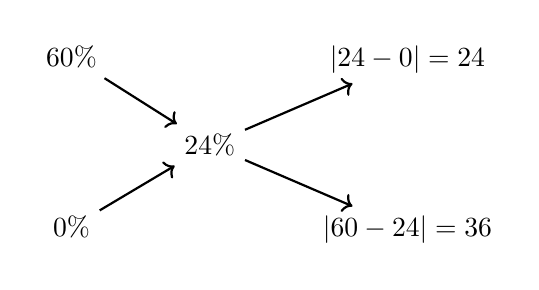
\begin{tikzpicture}
\matrix (m) [
    matrix of math nodes, 
    row sep=1.5em, 
    column sep=2.5em, 
    ampersand replacement=\&
  ] {
    60\% \&      \& \vert 24 - 0 \vert = 24 \\
         \& 24\% \& \\
    0\%  \&      \& \vert 60 - 24 \vert = 36 \\
  };
  % Pfeile von links zur Mitte
  \draw[->, thick] (m-1-1) -- (m-2-2);
  \draw[->, thick] (m-3-1) -- (m-2-2);

  % Pfeile von der Mitte nach rechts
  \draw[->, thick] (m-2-2) -- (m-1-3);
  \draw[->, thick] (m-2-2) -- (m-3-3);
\end{tikzpicture}
\pp



\begin{align*}
60~\text{Teile} ~&\hat{=}~ 1200 ~\text{g} \\
1~\text{Teil} ~&\hat{=}~ 20 ~\text{g} \\
36~\text{Teile} ~&\hat{=}~ 720 ~\text{g} \\
\end{align*}
\end{center}


\end{frame}



\begin{frame}
\begin{align*}
1200~\text{g} \cdot \frac{24}{60} &= 480~\text{g} \\
1200~\text{g} \cdot \frac{36}{60} &= 720 ~\text{g}
\end{align*}
\end{frame}






\begin{frame}
\begin{minipage}{.5\textwidth}


{\color{miugray}$\blacksquare ~$} \textbf{Aufgabe 4} \par \vspace*{2mm}

Wie viel kg 10\%ige Saccharose-Lösung müssen zu 100 kg 30 \%iger Saccharose-Lösung
gegeben werden, um eine 20\%ige Saccharose-Lösung zu erhalten? Berechnen Sie die Lösung
über die Mischungsgleichung.



\end{minipage}%
\hspace*{4mm}
\begin{minipage}{.5\textwidth}

\antwort{

Mit: $x_1 = 10\% $ ; $x_2 = 20\%$ ; $x_3 = 30\% $ ; $m_1 = ? $ ; $m_2 = m_3 + m_1$ ; $m_3 = 100$ 

\begin{align*}
\uncover<2->{m_3x_3 + m_1x_1 			&= m_3x_2 + m_1x_2 \\}
\uncover<3->{m_3x_3 + m_1x_1 - m_1x_2 	&= m_3x_2 \\}
\uncover<4->{m_1x_1 - m_1x_2 			&= m_3x_2 - m_3x_3 \\}
\uncover<5->{m_1(x_1 - x_2) 				&= m_3(x_2-x_3) \\}
\uncover<6->{m_1 						&= \frac{m_3(x_2-x_3)}{x_1 - x_2} \\}
\uncover<7->{m_1 						&= \frac{100(0,2-0,3)}{0,1 - 0,2} \\
&= 100}
\end{align*}
}



\end{minipage}%
\end{frame}


\begin{frame}

\begin{minipage}{.5\textwidth}


{\color{miugray}$\blacksquare ~$} \textbf{Aufgabe 5} \par \vspace*{2mm}
Für eine Mikrowellenfrequenz von 2450 MHz und eine Temperatur von \mbox{20 °C} beträgt die
stoffabhängige Permitivitätszahl $\varepsilon '$ von rohen Kartoffeln 64 und der Verlustwinkel tan $\delta$ 0,23.
Nehmen Sie als Lichtgeschwindigkeit den gerundeten Wert 3 * 10$^8$ m/s an.
Bestimmen Sie anhand untenstehender Formel die Eindringtiefe des Feldes in die
Kartoffel. Bestimmen Sie die Eindringtiefe auch für Wasser bei 25°C ($\varepsilon '$ 78; tan $\delta$: 0,16) und Eis
($\varepsilon '$: 3,2; tan $\delta$: 0,0009).

\begin{align*}
Z = \frac{\lambda}{2 \pi} \left[ \frac{2}{\varepsilon ' \cdot (\sqrt{1+ \tan^2 \delta} - 1)} \right]^{\frac{1}{2}}
\end{align*}
\pp

\end{minipage}%
\hspace*{4mm}
\begin{minipage}{.5\textwidth}
\antwort{
\only<1>{
Lambda berechnen: 
\begin{align*}
\lambda = \frac{c}{f} \qquad \rightarrow \qquad \frac{3 \cdot 10^8 ~\text{m/s}}{2.450 \cdot 10^6 ~\text{Hz}} = 0,1224 ~\text{m}
\end{align*}
}
\uncover<2->{
Kartoffel:
\begin{align*}
Z &= \frac{0,1224 ~\text{m}}{2 \pi} \left[ \frac{2}{64 \cdot (\sqrt{1+ (0,23)^2} - 1)} \right]^{\frac{1}{2}} \\
 &= 0,0213 ~\text{m}
\end{align*}
}

\uncover<3->{
Wasser:
\begin{align*}
Z &= \frac{0,1224 ~\text{m}}{2 \pi} \left[ \frac{2}{78 \cdot (\sqrt{1+ (0,16)^2} - 1)} \right]^{\frac{1}{2}} \\
 &= 0,0276 ~\text{m}
\end{align*}
}

\uncover<4->{
Eis:
\begin{align*}
Z &= \frac{0,1224 ~\text{m}}{2 \pi} \left[ \frac{2}{3,2 \cdot (\sqrt{1+ (0,0009)^2} - 1)} \right]^{\frac{1}{2}} \\
 &= 24,2 ~\text{m}
\end{align*}
}

}

\end{minipage}%

\end{frame}


\begin{frame}
\begin{minipage}{.5\textwidth}


{\color{miugray}$\blacksquare ~$} \textbf{Aufgabe 5} \par \vspace*{2mm}

Wie ist die Eindringtiefe Z definiert?


\end{minipage}%
\hspace*{4mm}
\begin{minipage}{.5\textwidth}
\antwort{
\uncover<2->{
\textbf{Eindringtiefe Z:} \par Punkt, an dem die elektrische Feldstärke nur noch 1/e von der ursprünglichen Feldstärke entspricht.
}
}

\end{minipage}%
\end{frame}



\end{document}
